\documentclass{standalone}

%----------------------------------------------------------------------------------------------%
%                                 Packages and basic declarations
%----------------------------------------------------------------------------------------------%

\usepackage[utf8]{inputenc}
\usepackage{pgfplots}
\usepackage{tikz}


%----------------------------------------------------------------------------------------------%
%----------------------------------------------------------------------------------------------%
%                                            DOCUMENT STARTS
%----------------------------------------------------------------------------------------------%
%----------------------------------------------------------------------------------------------%

\begin{document}


%Tikz picture starts%

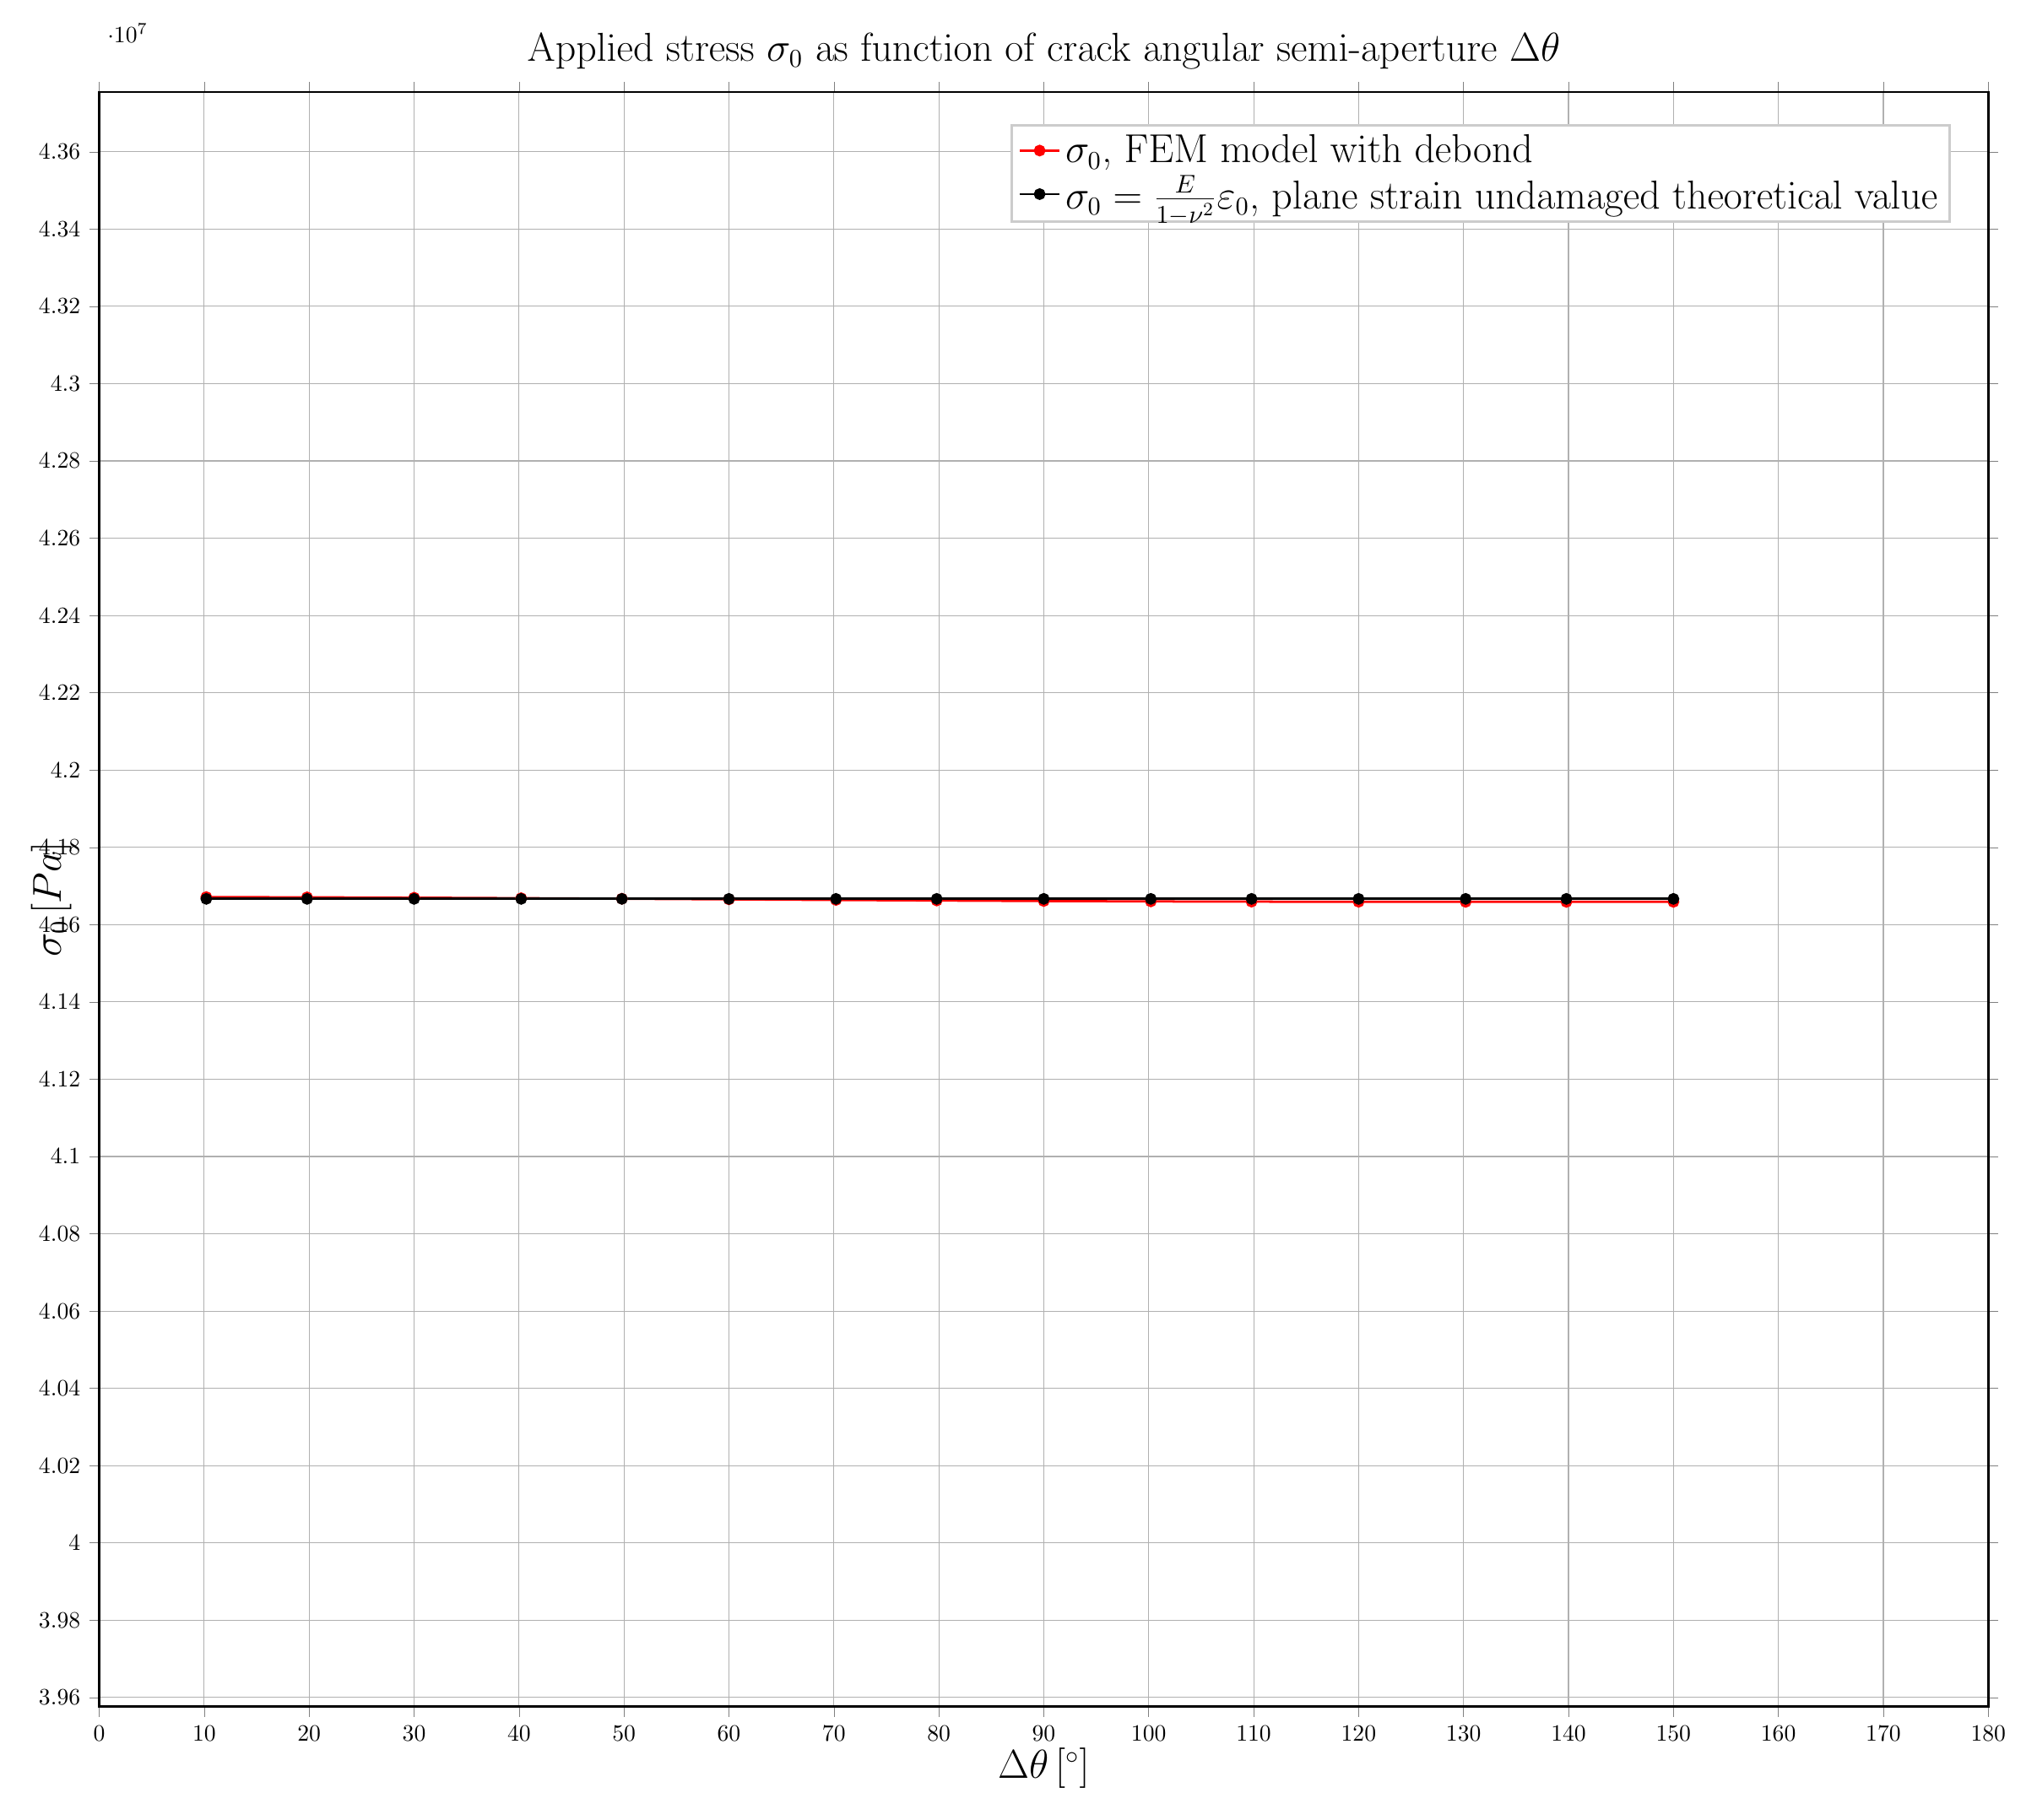
\begin{tikzpicture}

%Tikz axis starts%

\begin{axis}[width=30cm,
title={Applied stress $\sigma_{0}$ as function of crack angular semi-aperture  $\Delta\theta$},
title style={font=\fontsize{16}{8}\selectfont},
xlabel style={at={(axis description cs:0.5,-0.02)},anchor=north,font=\fontsize{16}{8}\selectfont},
ylabel style={at={(axis description cs:-0.01,.5)},anchor=south,font=\fontsize{16}{8}\selectfont},
xlabel={$\Delta\theta\left[^{\circ}\right]$},ylabel={$\sigma_{0}\left[Pa\right]$},
xmin=0.0,
xmax=180.0,
ymin=39576002.4494,
ymax=43754819.3263,
tick align=outside,
tick label style={font=\normalsize},
xtick={0.0,10.0,20.0,30.0,40.0,50.0,60.0,70.0,80.0,90.0,100.0,110.0,120.0,130.0,140.0,150.0,160.0,170.0,180.0},
xmajorgrids,
x grid style={lightgray!92.026143790849673!black},
ymajorgrids,
y grid style={lightgray!92.026143790849673!black},
line width=0.35mm,
legend style={draw=white!80.0!black,font=\fontsize{16}{12}\selectfont},
legend entries={{$\sigma_{0}$, FEM model with debond},{$\sigma_{0}=\frac{E}{1-\nu^{2}}\varepsilon_{0}$, plane strain undamaged theoretical value}},
legend cell align={left}
]

\addplot[red,smooth,mark=*]
table{
10.1996888272 41671256.5012
19.800125885 41670673.5346
29.9998676461 41669696.9215
40.1999526243 41668423.1158
49.8000464651 41667035.5007
60.0001314432 41665456.2919
70.1998714969 41663866.9147
79.8003102622 41662454.1377
90.0000025045 41661155.9028
100.199687917 41660162.6289
109.800126682 41659536.3743
119.999866736 41659162.9256
130.199948299 41659006.4851
139.800052385 41658967.0497
150.000133948 41658963.475
};

\addplot[black,smooth,mark=*]
table{
10.1996888272 41666666.6667
19.800125885 41666666.6667
29.9998676461 41666666.6667
40.1999526243 41666666.6667
49.8000464651 41666666.6667
60.0001314432 41666666.6667
70.1998714969 41666666.6667
79.8003102622 41666666.6667
90.0000025045 41666666.6667
100.199687917 41666666.6667
109.800126682 41666666.6667
119.999866736 41666666.6667
130.199948299 41666666.6667
139.800052385 41666666.6667
150.000133948 41666666.6667
};

\end{axis}
%Tikz axis ends%


\end{tikzpicture}
%Tikz picture ends%


\end{document}

%----------------------------------------------------------------------------------------------%
%----------------------------------------------------------------------------------------------%
%                                            DOCUMENT ENDS
%----------------------------------------------------------------------------------------------%
%----------------------------------------------------------------------------------------------%

